\documentclass[1p]{elsarticle_modified}
%\bibliographystyle{elsarticle-num}

%\usepackage[colorlinks]{hyperref}
%\usepackage{abbrmath_seonhwa} %\Abb, \Ascr, \Acal ,\Abf, \Afrak
\usepackage{amsfonts}
\usepackage{amssymb}
\usepackage{amsmath}
\usepackage{amsthm}
\usepackage{scalefnt}
\usepackage{amsbsy}
\usepackage{kotex}
\usepackage{caption}
\usepackage{subfig}
\usepackage{color}
\usepackage{graphicx}
\usepackage{xcolor} %% white, black, red, green, blue, cyan, magenta, yellow
\usepackage{float}
\usepackage{setspace}
\usepackage{hyperref}

\usepackage{tikz}
\usetikzlibrary{arrows}

\usepackage{multirow}
\usepackage{array} % fixed length table
\usepackage{hhline}

%%%%%%%%%%%%%%%%%%%%%
\makeatletter
\renewcommand*\env@matrix[1][\arraystretch]{%
	\edef\arraystretch{#1}%
	\hskip -\arraycolsep
	\let\@ifnextchar\new@ifnextchar
	\array{*\c@MaxMatrixCols c}}
\makeatother %https://tex.stackexchange.com/questions/14071/how-can-i-increase-the-line-spacing-in-a-matrix
%%%%%%%%%%%%%%%

\usepackage[normalem]{ulem}

\newcommand{\msout}[1]{\ifmmode\text{\sout{\ensuremath{#1}}}\else\sout{#1}\fi}
%SOURCE: \msout is \stkout macro in https://tex.stackexchange.com/questions/20609/strikeout-in-math-mode

\newcommand{\cancel}[1]{
	\ifmmode
	{\color{red}\msout{#1}}
	\else
	{\color{red}\sout{#1}}
	\fi
}

\newcommand{\add}[1]{
	{\color{blue}\uwave{#1}}
}

\newcommand{\replace}[2]{
	\ifmmode
	{\color{red}\msout{#1}}{\color{blue}\uwave{#2}}
	\else
	{\color{red}\sout{#1}}{\color{blue}\uwave{#2}}
	\fi
}

\newcommand{\Sol}{\mathcal{S}} %segment
\newcommand{\D}{D} %diagram
\newcommand{\A}{\mathcal{A}} %arc


%%%%%%%%%%%%%%%%%%%%%%%%%%%%%5 test

\def\sl{\operatorname{\textup{SL}}(2,\Cbb)}
\def\psl{\operatorname{\textup{PSL}}(2,\Cbb)}
\def\quan{\mkern 1mu \triangleright \mkern 1mu}

\theoremstyle{definition}
\newtheorem{thm}{Theorem}[section]
\newtheorem{prop}[thm]{Proposition}
\newtheorem{lem}[thm]{Lemma}
\newtheorem{ques}[thm]{Question}
\newtheorem{cor}[thm]{Corollary}
\newtheorem{defn}[thm]{Definition}
\newtheorem{exam}[thm]{Example}
\newtheorem{rmk}[thm]{Remark}
\newtheorem{alg}[thm]{Algorithm}

\newcommand{\I}{\sqrt{-1}}
\begin{document}

%\begin{frontmatter}
%
%\title{Boundary parabolic representations of knots up to 8 crossings}
%
%%% Group authors per affiliation:
%\author{Yunhi Cho} 
%\address{Department of Mathematics, University of Seoul, Seoul, Korea}
%\ead{yhcho@uos.ac.kr}
%
%
%\author{Seonhwa Kim} %\fnref{s_kim}}
%\address{Center for Geometry and Physics, Institute for Basic Science, Pohang, 37673, Korea}
%\ead{ryeona17@ibs.re.kr}
%
%\author{Hyuk Kim}
%\address{Department of Mathematical Sciences, Seoul National University, Seoul 08826, Korea}
%\ead{hyukkim@snu.ac.kr}
%
%\author{Seokbeom Yoon}
%\address{Department of Mathematical Sciences, Seoul National University, Seoul, 08826,  Korea}
%\ead{sbyoon15@snu.ac.kr}
%
%\begin{abstract}
%We find all boundary parabolic representation of knots up to 8 crossings.
%
%\end{abstract}
%\begin{keyword}
%    \MSC[2010] 57M25 
%\end{keyword}
%
%\end{frontmatter}

%\linenumbers
%\tableofcontents
%
\newcommand\colored[1]{\textcolor{white}{\rule[-0.35ex]{0.8em}{1.4ex}}\kern-0.8em\color{red} #1}%
%\newcommand\colored[1]{\textcolor{white}{ #1}\kern-2.17ex	\textcolor{white}{ #1}\kern-1.81ex	\textcolor{white}{ #1}\kern-2.15ex\color{red}#1	}

{\Large $\underline{12n_{0034}~(K12n_{0034})}$}

\setlength{\tabcolsep}{10pt}
\renewcommand{\arraystretch}{1.6}
\vspace{1cm}\begin{tabular}{m{100pt}>{\centering\arraybackslash}m{274pt}}
\multirow{5}{120pt}{
	\centering
	\includegraphics[width=112pt]{../../../GIT/diagram.site/Diagrams/png/2123_12n_0034.png}\\
\ \ \ A knot diagram\footnotemark}&
\allowdisplaybreaks
\textbf{Linearized knot diagam} \\
\cline{2-2}
 &
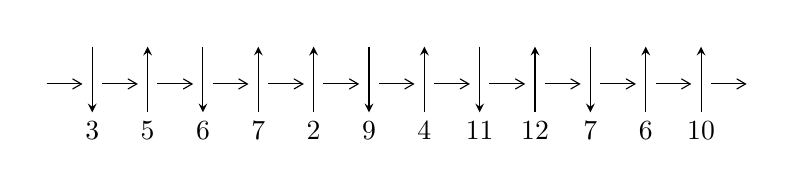
\begin{tikzpicture}[x=20pt, y=17pt]
	% nodes
	\node (C0) at (0, 0) {};
	\node (C1) at (1, 0) {};
	\node (C1U) at (1, +1) {};
	\node (C1D) at (1, -1) {3};

	\node (C2) at (2, 0) {};
	\node (C2U) at (2, +1) {};
	\node (C2D) at (2, -1) {5};

	\node (C3) at (3, 0) {};
	\node (C3U) at (3, +1) {};
	\node (C3D) at (3, -1) {6};

	\node (C4) at (4, 0) {};
	\node (C4U) at (4, +1) {};
	\node (C4D) at (4, -1) {7};

	\node (C5) at (5, 0) {};
	\node (C5U) at (5, +1) {};
	\node (C5D) at (5, -1) {2};

	\node (C6) at (6, 0) {};
	\node (C6U) at (6, +1) {};
	\node (C6D) at (6, -1) {9};

	\node (C7) at (7, 0) {};
	\node (C7U) at (7, +1) {};
	\node (C7D) at (7, -1) {4};

	\node (C8) at (8, 0) {};
	\node (C8U) at (8, +1) {};
	\node (C8D) at (8, -1) {11};

	\node (C9) at (9, 0) {};
	\node (C9U) at (9, +1) {};
	\node (C9D) at (9, -1) {12};

	\node (C10) at (10, 0) {};
	\node (C10U) at (10, +1) {};
	\node (C10D) at (10, -1) {7};

	\node (C11) at (11, 0) {};
	\node (C11U) at (11, +1) {};
	\node (C11D) at (11, -1) {6};

	\node (C12) at (12, 0) {};
	\node (C12U) at (12, +1) {};
	\node (C12D) at (12, -1) {10};
	\node (C13) at (13, 0) {};

	% arrows
	\draw[->,>={angle 60}]
	(C0) edge (C1) (C1) edge (C2) (C2) edge (C3) (C3) edge (C4) (C4) edge (C5) (C5) edge (C6) (C6) edge (C7) (C7) edge (C8) (C8) edge (C9) (C9) edge (C10) (C10) edge (C11) (C11) edge (C12) (C12) edge (C13) ;	\draw[->,>=stealth]
	(C1U) edge (C1D) (C2D) edge (C2U) (C3U) edge (C3D) (C4D) edge (C4U) (C5D) edge (C5U) (C6U) edge (C6D) (C7D) edge (C7U) (C8U) edge (C8D) (C9D) edge (C9U) (C10U) edge (C10D) (C11D) edge (C11U) (C12D) edge (C12U) ;
	\end{tikzpicture} \\
\hhline{~~} \\& 
\textbf{Solving Sequence} \\ \cline{2-2} 
 &
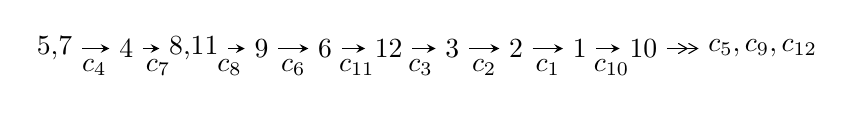
\begin{tikzpicture}[x=23pt, y=7pt]
	% node
	\node (A0) at (-1/8, 0) {5,7};
	\node (A1) at (1, 0) {4};
	\node (A2) at (33/16, 0) {8,11};
	\node (A3) at (25/8, 0) {9};
	\node (A4) at (33/8, 0) {6};
	\node (A5) at (41/8, 0) {12};
	\node (A6) at (49/8, 0) {3};
	\node (A7) at (57/8, 0) {2};
	\node (A8) at (65/8, 0) {1};
	\node (A9) at (73/8, 0) {10};
	\node (C1) at (1/2, -1) {$c_{4}$};
	\node (C2) at (3/2, -1) {$c_{7}$};
	\node (C3) at (21/8, -1) {$c_{8}$};
	\node (C4) at (29/8, -1) {$c_{6}$};
	\node (C5) at (37/8, -1) {$c_{11}$};
	\node (C6) at (45/8, -1) {$c_{3}$};
	\node (C7) at (53/8, -1) {$c_{2}$};
	\node (C8) at (61/8, -1) {$c_{1}$};
	\node (C9) at (69/8, -1) {$c_{10}$};
	\node (A10) at (11, 0) {$c_{5},c_{9},c_{12}$};

	% edge
	\draw[->,>=stealth]	
	(A0) edge (A1) (A1) edge (A2) (A2) edge (A3) (A3) edge (A4) (A4) edge (A5) (A5) edge (A6) (A6) edge (A7) (A7) edge (A8) (A8) edge (A9) ;
	\draw[->>,>={angle 60}]	
	(A9) edge (A10);
\end{tikzpicture} \\ 

\end{tabular} \\

\footnotetext{
The image of knot diagram is generated by the software ``\textbf{Draw programme}" developed by Andrew Bartholomew(\url{http://www.layer8.co.uk/maths/draw/index.htm\#Running-draw}), where we modified some parts for our purpose(\url{https://github.com/CATsTAILs/LinksPainter}).
}\phantom \\ \newline 
\centering \textbf{Ideals for irreducible components\footnotemark of $X_{\text{par}}$} 
 
\begin{align*}
I^u_{1}&=\langle 
1.80347\times10^{133} u^{37}-4.04668\times10^{133} u^{36}+\cdots+1.44050\times10^{137} b+7.58135\times10^{136},\\
\phantom{I^u_{1}}&\phantom{= \langle  }2.78701\times10^{134} u^{37}-5.34254\times10^{134} u^{36}+\cdots+2.01671\times10^{138} a+5.65465\times10^{138},\\
\phantom{I^u_{1}}&\phantom{= \langle  }u^{38}-2 u^{37}+\cdots+12288 u+4096\rangle \\
I^u_{2}&=\langle 
u^3- u^2+b+2 u,\;- u^2+a+u-1,\;u^4+u^2+u+1\rangle \\
I^u_{3}&=\langle 
3 u^5- u^4+5 u^3-3 u^2+b+4 u-4,\;2 u^5+3 u^3- u^2+a+2 u-2,\;u^6- u^5+2 u^4-2 u^3+2 u^2-2 u+1\rangle \\
\\
I^v_{1}&=\langle 
a,\;-963772 v^{11}+658631 v^{10}+\cdots+707733 b+3141326,\\
\phantom{I^v_{1}}&\phantom{= \langle  }v^{12}- v^{11}-4 v^{10}-5 v^9+19 v^8+9 v^7-31 v^6+29 v^5+31 v^4-18 v^3+3 v^2-3 v+1\rangle \\
\end{align*}
\raggedright * 4 irreducible components of $\dim_{\mathbb{C}}=0$, with total 60 representations.\\
\footnotetext{All coefficients of polynomials are rational numbers. But the coefficients are sometimes approximated in decimal forms when there is not enough margin.}
\newpage
\renewcommand{\arraystretch}{1}
\centering \section*{I. $I^u_{1}= \langle 1.80\times10^{133} u^{37}-4.05\times10^{133} u^{36}+\cdots+1.44\times10^{137} b+7.58\times10^{136},\;2.79\times10^{134} u^{37}-5.34\times10^{134} u^{36}+\cdots+2.02\times10^{138} a+5.65\times10^{138},\;u^{38}-2 u^{37}+\cdots+12288 u+4096 \rangle$}
\flushleft \textbf{(i) Arc colorings}\\
\begin{tabular}{m{7pt} m{180pt} m{7pt} m{180pt} }
\flushright $a_{5}=$&$\begin{pmatrix}1\\0\end{pmatrix}$ \\
\flushright $a_{7}=$&$\begin{pmatrix}0\\u\end{pmatrix}$ \\
\flushright $a_{4}=$&$\begin{pmatrix}1\\u^2\end{pmatrix}$ \\
\flushright $a_{8}=$&$\begin{pmatrix}u\\u^3+u\end{pmatrix}$ \\
\flushright $a_{11}=$&$\begin{pmatrix}-0.000138196 u^{37}+0.000264914 u^{36}+\cdots+2.22627 u-2.80391\\-0.000125197 u^{37}+0.000280921 u^{36}+\cdots+3.09647 u-0.526298\end{pmatrix}$ \\
\flushright $a_{9}=$&$\begin{pmatrix}-0.0000643751 u^{37}+0.000175800 u^{36}+\cdots-4.14636 u+0.169342\\0.0000210320 u^{37}-0.0000415391 u^{36}+\cdots-0.351856 u-0.288364\end{pmatrix}$ \\
\flushright $a_{6}=$&$\begin{pmatrix}0.0000103293 u^{37}+5.50817\times10^{-6} u^{36}+\cdots+0.765170 u+1.22937\\-0.0000463037 u^{37}+0.0000938416 u^{36}+\cdots+0.102969 u-0.0432937\end{pmatrix}$ \\
\flushright $a_{12}=$&$\begin{pmatrix}-0.000154935 u^{37}+0.000266148 u^{36}+\cdots+3.91415 u-3.54515\\-0.000183169 u^{37}+0.000395135 u^{36}+\cdots+2.91568 u-0.405958\end{pmatrix}$ \\
\flushright $a_{3}=$&$\begin{pmatrix}0.0000125731 u^{37}-0.0000323095 u^{36}+\cdots-0.598837 u+0.850308\\0.0000180956 u^{37}-0.0000598188 u^{36}+\cdots-0.780260 u-0.190793\end{pmatrix}$ \\
\flushright $a_{2}=$&$\begin{pmatrix}-5.52255\times10^{-6} u^{37}+0.0000275093 u^{36}+\cdots+0.181423 u+1.04110\\0.0000180956 u^{37}-0.0000598188 u^{36}+\cdots-0.780260 u-0.190793\end{pmatrix}$ \\
\flushright $a_{1}=$&$\begin{pmatrix}0.0000555017 u^{37}-0.0000873032 u^{36}+\cdots+0.298354 u+1.16548\\0.0000451724 u^{37}-0.0000928114 u^{36}+\cdots-0.466816 u-0.0638856\end{pmatrix}$ \\
\flushright $a_{10}=$&$\begin{pmatrix}-0.000138196 u^{37}+0.000264914 u^{36}+\cdots+2.22627 u-2.80391\\-0.000147500 u^{37}+0.000324572 u^{36}+\cdots+2.38937 u-0.573314\end{pmatrix}$\\&\end{tabular}
\flushleft \textbf{(ii) Obstruction class $= -1$}\\~\\
\flushleft \textbf{(iii) Cusp Shapes $= -0.000218010 u^{37}+0.000603676 u^{36}+\cdots-22.4576 u-0.864966$}\\~\\
\newpage\renewcommand{\arraystretch}{1}
\flushleft \textbf{(iv) u-Polynomials at the component}\newline \\
\begin{tabular}{m{50pt}|m{274pt}}
Crossings & \hspace{64pt}u-Polynomials at each crossing \\
\hline $$\begin{aligned}c_{1}\end{aligned}$$&$\begin{aligned}
&u^{38}+28 u^{37}+\cdots+159 u+1
\end{aligned}$\\
\hline $$\begin{aligned}c_{2},c_{5}\end{aligned}$$&$\begin{aligned}
&u^{38}+8 u^{37}+\cdots+11 u+1
\end{aligned}$\\
\hline $$\begin{aligned}c_{3}\end{aligned}$$&$\begin{aligned}
&u^{38}-8 u^{37}+\cdots+17360 u+1732
\end{aligned}$\\
\hline $$\begin{aligned}c_{4},c_{7}\end{aligned}$$&$\begin{aligned}
&u^{38}+2 u^{37}+\cdots-12288 u+4096
\end{aligned}$\\
\hline $$\begin{aligned}c_{6}\end{aligned}$$&$\begin{aligned}
&u^{38}-4 u^{37}+\cdots-3 u+1
\end{aligned}$\\
\hline $$\begin{aligned}c_{8}\end{aligned}$$&$\begin{aligned}
&u^{38}-3 u^{37}+\cdots-11264 u+1024
\end{aligned}$\\
\hline $$\begin{aligned}c_{9},c_{12}\end{aligned}$$&$\begin{aligned}
&u^{38}+13 u^{37}+\cdots+8 u+1
\end{aligned}$\\
\hline $$\begin{aligned}c_{10}\end{aligned}$$&$\begin{aligned}
&u^{38}+2 u^{37}+\cdots+575973 u+248449
\end{aligned}$\\
\hline $$\begin{aligned}c_{11}\end{aligned}$$&$\begin{aligned}
&u^{38}+8 u^{37}+\cdots-149993 u+47809
\end{aligned}$\\
\hline
\end{tabular}\\~\\
\newpage\renewcommand{\arraystretch}{1}
\flushleft \textbf{(v) Riley Polynomials at the component}\newline \\
\begin{tabular}{m{50pt}|m{274pt}}
Crossings & \hspace{64pt}Riley Polynomials at each crossing \\
\hline $$\begin{aligned}c_{1}\end{aligned}$$&$\begin{aligned}
&y^{38}-28 y^{37}+\cdots-10893 y+1
\end{aligned}$\\
\hline $$\begin{aligned}c_{2},c_{5}\end{aligned}$$&$\begin{aligned}
&y^{38}+28 y^{37}+\cdots+159 y+1
\end{aligned}$\\
\hline $$\begin{aligned}c_{3}\end{aligned}$$&$\begin{aligned}
&y^{38}-84 y^{37}+\cdots+436784552 y+2999824
\end{aligned}$\\
\hline $$\begin{aligned}c_{4},c_{7}\end{aligned}$$&$\begin{aligned}
&y^{38}+70 y^{37}+\cdots+134217728 y+16777216
\end{aligned}$\\
\hline $$\begin{aligned}c_{6}\end{aligned}$$&$\begin{aligned}
&y^{38}+4 y^{37}+\cdots+19 y+1
\end{aligned}$\\
\hline $$\begin{aligned}c_{8}\end{aligned}$$&$\begin{aligned}
&y^{38}-69 y^{37}+\cdots-7864320 y+1048576
\end{aligned}$\\
\hline $$\begin{aligned}c_{9},c_{12}\end{aligned}$$&$\begin{aligned}
&y^{38}+y^{37}+\cdots-84 y+1
\end{aligned}$\\
\hline $$\begin{aligned}c_{10}\end{aligned}$$&$\begin{aligned}
&y^{38}-84 y^{37}+\cdots+1086486467931 y+61726905601
\end{aligned}$\\
\hline $$\begin{aligned}c_{11}\end{aligned}$$&$\begin{aligned}
&y^{38}+48 y^{37}+\cdots+51838210455 y+2285700481
\end{aligned}$\\
\hline
\end{tabular}\\~\\
\newpage\flushleft \textbf{(vi) Complex Volumes and Cusp Shapes}
$$\begin{array}{c|c|c}  
\text{Solutions to }I^u_{1}& \I (\text{vol} + \sqrt{-1}CS) & \text{Cusp shape}\\
 \hline 
\begin{aligned}
u &= \phantom{-}0.269512 + 0.935520 I \\
a &= -0.458289 - 0.782512 I \\
b &= \phantom{-}0.677405 + 0.518877 I\end{aligned}
 & -0.61516 + 8.47206 I & -1.23185 - 12.18265 I \\ \hline\begin{aligned}
u &= \phantom{-}0.269512 - 0.935520 I \\
a &= -0.458289 + 0.782512 I \\
b &= \phantom{-}0.677405 - 0.518877 I\end{aligned}
 & -0.61516 - 8.47206 I & -1.23185 + 12.18265 I \\ \hline\begin{aligned}
u &= -0.615656 + 0.694581 I \\
a &= -0.427914 + 0.398057 I \\
b &= \phantom{-}0.267942 + 0.980799 I\end{aligned}
 & \phantom{-}1.12636 - 1.44186 I & \phantom{-}2.40380 + 3.54555 I \\ \hline\begin{aligned}
u &= -0.615656 - 0.694581 I \\
a &= -0.427914 - 0.398057 I \\
b &= \phantom{-}0.267942 - 0.980799 I\end{aligned}
 & \phantom{-}1.12636 + 1.44186 I & \phantom{-}2.40380 - 3.54555 I \\ \hline\begin{aligned}
u &= -0.690714 + 0.617908 I \\
a &= -0.599875 - 0.724392 I \\
b &= -0.695539 + 0.625151 I\end{aligned}
 & \phantom{-}0.91553 - 4.18220 I & \phantom{-}3.10264 + 7.31279 I \\ \hline\begin{aligned}
u &= -0.690714 - 0.617908 I \\
a &= -0.599875 + 0.724392 I \\
b &= -0.695539 - 0.625151 I\end{aligned}
 & \phantom{-}0.91553 + 4.18220 I & \phantom{-}3.10264 - 7.31279 I \\ \hline\begin{aligned}
u &= -0.962152 + 0.487944 I \\
a &= \phantom{-}0.020845 + 0.197190 I \\
b &= -0.32060 + 1.60868 I\end{aligned}
 & \phantom{-}0.067821 + 0.704860 I & \phantom{-}1.59983 - 2.96425 I \\ \hline\begin{aligned}
u &= -0.962152 - 0.487944 I \\
a &= \phantom{-}0.020845 - 0.197190 I \\
b &= -0.32060 - 1.60868 I\end{aligned}
 & \phantom{-}0.067821 - 0.704860 I & \phantom{-}1.59983 + 2.96425 I \\ \hline\begin{aligned}
u &= \phantom{-}0.334991 + 0.821597 I \\
a &= -0.428276 + 0.927379 I \\
b &= -0.299801 - 0.583140 I\end{aligned}
 & -3.35491 - 0.78621 I & -8.48784 + 2.29609 I \\ \hline\begin{aligned}
u &= \phantom{-}0.334991 - 0.821597 I \\
a &= -0.428276 - 0.927379 I \\
b &= -0.299801 + 0.583140 I\end{aligned}
 & -3.35491 + 0.78621 I & -8.48784 - 2.29609 I\\
 \hline 
 \end{array}$$\newpage$$\begin{array}{c|c|c}  
\text{Solutions to }I^u_{1}& \I (\text{vol} + \sqrt{-1}CS) & \text{Cusp shape}\\
 \hline 
\begin{aligned}
u &= \phantom{-}0.730737 + 0.068723 I \\
a &= \phantom{-}0.810489 + 0.363992 I \\
b &= \phantom{-}1.45774 + 1.16856 I\end{aligned}
 & -0.42860 - 2.78462 I & \phantom{-}1.78865 + 4.97070 I \\ \hline\begin{aligned}
u &= \phantom{-}0.730737 - 0.068723 I \\
a &= \phantom{-}0.810489 - 0.363992 I \\
b &= \phantom{-}1.45774 - 1.16856 I\end{aligned}
 & -0.42860 + 2.78462 I & \phantom{-}1.78865 - 4.97070 I \\ \hline\begin{aligned}
u &= \phantom{-}0.154768 + 0.641440 I \\
a &= -0.858708 + 0.997854 I \\
b &= \phantom{-}0.415361 - 0.487054 I\end{aligned}
 & -1.32113 - 1.32492 I & -1.95750 + 1.98412 I \\ \hline\begin{aligned}
u &= \phantom{-}0.154768 - 0.641440 I \\
a &= -0.858708 - 0.997854 I \\
b &= \phantom{-}0.415361 + 0.487054 I\end{aligned}
 & -1.32113 + 1.32492 I & -1.95750 - 1.98412 I \\ \hline\begin{aligned}
u &= \phantom{-}1.336190 + 0.226899 I \\
a &= \phantom{-}0.552450 + 0.930807 I \\
b &= \phantom{-}0.80282 + 3.46642 I\end{aligned}
 & -0.61371 - 2.86891 I & -0.25435 + 4.83204 I \\ \hline\begin{aligned}
u &= \phantom{-}1.336190 - 0.226899 I \\
a &= \phantom{-}0.552450 - 0.930807 I \\
b &= \phantom{-}0.80282 - 3.46642 I\end{aligned}
 & -0.61371 + 2.86891 I & -0.25435 - 4.83204 I \\ \hline\begin{aligned}
u &= \phantom{-}0.300084 + 0.412662 I \\
a &= \phantom{-}0.10831 + 2.92562 I \\
b &= -0.16429 + 3.48640 I\end{aligned}
 & \phantom{-}1.67684 - 2.65330 I & \phantom{-}7.7232 - 16.8130 I \\ \hline\begin{aligned}
u &= \phantom{-}0.300084 - 0.412662 I \\
a &= \phantom{-}0.10831 - 2.92562 I \\
b &= -0.16429 - 3.48640 I\end{aligned}
 & \phantom{-}1.67684 + 2.65330 I & \phantom{-}7.7232 + 16.8130 I \\ \hline\begin{aligned}
u &= -0.392217 + 0.325280 I \\
a &= -1.29311 + 2.21775 I \\
b &= -0.16047 + 3.66337 I\end{aligned}
 & \phantom{-}2.15015 - 1.46241 I & -0.02794 + 14.08993 I \\ \hline\begin{aligned}
u &= -0.392217 - 0.325280 I \\
a &= -1.29311 - 2.21775 I \\
b &= -0.16047 - 3.66337 I\end{aligned}
 & \phantom{-}2.15015 + 1.46241 I & -0.02794 - 14.08993 I\\
 \hline 
 \end{array}$$\newpage$$\begin{array}{c|c|c}  
\text{Solutions to }I^u_{1}& \I (\text{vol} + \sqrt{-1}CS) & \text{Cusp shape}\\
 \hline 
\begin{aligned}
u &= -0.209980 + 0.250980 I \\
a &= -3.00779 + 0.52768 I \\
b &= -0.802018 + 0.832176 I\end{aligned}
 & \phantom{-}1.91078 - 0.79833 I & \phantom{-}4.44525 - 0.45789 I \\ \hline\begin{aligned}
u &= -0.209980 - 0.250980 I \\
a &= -3.00779 - 0.52768 I \\
b &= -0.802018 - 0.832176 I\end{aligned}
 & \phantom{-}1.91078 + 0.79833 I & \phantom{-}4.44525 + 0.45789 I \\ \hline\begin{aligned}
u &= -1.10703 + 1.69579 I \\
a &= \phantom{-}0.928872 - 0.073456 I \\
b &= -2.06666 - 3.80312 I\end{aligned}
 & -6.26733 + 3.08288 I & \phantom{-0.000000 } 0 \\ \hline\begin{aligned}
u &= -1.10703 - 1.69579 I \\
a &= \phantom{-}0.928872 + 0.073456 I \\
b &= -2.06666 + 3.80312 I\end{aligned}
 & -6.26733 - 3.08288 I & \phantom{-0.000000 } 0 \\ \hline\begin{aligned}
u &= \phantom{-}0.41366 + 2.27352 I \\
a &= \phantom{-}0.273778 - 1.053910 I \\
b &= \phantom{-}0.83748 + 3.68747 I\end{aligned}
 & -12.39510 + 1.09723 I & \phantom{-0.000000 } 0 \\ \hline\begin{aligned}
u &= \phantom{-}0.41366 - 2.27352 I \\
a &= \phantom{-}0.273778 + 1.053910 I \\
b &= \phantom{-}0.83748 - 3.68747 I\end{aligned}
 & -12.39510 - 1.09723 I & \phantom{-0.000000 } 0 \\ \hline\begin{aligned}
u &= -0.98102 + 2.10542 I \\
a &= -0.285160 - 1.017430 I \\
b &= -3.48637 + 2.72417 I\end{aligned}
 & -16.2164 - 7.5794 I & \phantom{-0.000000 } 0 \\ \hline\begin{aligned}
u &= -0.98102 - 2.10542 I \\
a &= -0.285160 + 1.017430 I \\
b &= -3.48637 - 2.72417 I\end{aligned}
 & -16.2164 + 7.5794 I & \phantom{-0.000000 } 0 \\ \hline\begin{aligned}
u &= \phantom{-}1.14222 + 2.13195 I \\
a &= -0.006500 + 1.260510 I \\
b &= -6.15185 - 1.87143 I\end{aligned}
 & -15.9377 + 14.9717 I & \phantom{-0.000000 } 0 \\ \hline\begin{aligned}
u &= \phantom{-}1.14222 - 2.13195 I \\
a &= -0.006500 - 1.260510 I \\
b &= -6.15185 + 1.87143 I\end{aligned}
 & -15.9377 - 14.9717 I & \phantom{-0.000000 } 0\\
 \hline 
 \end{array}$$\newpage$$\begin{array}{c|c|c}  
\text{Solutions to }I^u_{1}& \I (\text{vol} + \sqrt{-1}CS) & \text{Cusp shape}\\
 \hline 
\begin{aligned}
u &= -0.58138 + 2.41986 I \\
a &= -0.021457 + 1.260750 I \\
b &= \phantom{-}3.60201 - 4.67413 I\end{aligned}
 & -12.2225 - 8.2203 I & \phantom{-0.000000 } 0 \\ \hline\begin{aligned}
u &= -0.58138 - 2.41986 I \\
a &= -0.021457 - 1.260750 I \\
b &= \phantom{-}3.60201 + 4.67413 I\end{aligned}
 & -12.2225 + 8.2203 I & \phantom{-0.000000 } 0 \\ \hline\begin{aligned}
u &= \phantom{-}1.75400 + 1.85534 I \\
a &= \phantom{-}1.163960 + 0.099561 I \\
b &= -0.64784 + 7.80385 I\end{aligned}
 & -6.74677 + 2.59569 I & \phantom{-0.000000 } 0 \\ \hline\begin{aligned}
u &= \phantom{-}1.75400 - 1.85534 I \\
a &= \phantom{-}1.163960 - 0.099561 I \\
b &= -0.64784 - 7.80385 I\end{aligned}
 & -6.74677 - 2.59569 I & \phantom{-0.000000 } 0 \\ \hline\begin{aligned}
u &= \phantom{-}0.32782 + 2.75595 I \\
a &= -0.238367 - 1.046580 I \\
b &= \phantom{-}3.58759 + 5.29844 I\end{aligned}
 & -17.5824 + 5.0951 I & \phantom{-0.000000 } 0 \\ \hline\begin{aligned}
u &= \phantom{-}0.32782 - 2.75595 I \\
a &= -0.238367 + 1.046580 I \\
b &= \phantom{-}3.58759 - 5.29844 I\end{aligned}
 & -17.5824 - 5.0951 I & \phantom{-0.000000 } 0 \\ \hline\begin{aligned}
u &= -0.22384 + 3.07549 I \\
a &= \phantom{-}0.016754 + 1.242340 I \\
b &= \phantom{-}1.64709 - 9.59445 I\end{aligned}
 & -17.7767 + 1.7959 I & \phantom{-0.000000 } 0 \\ \hline\begin{aligned}
u &= -0.22384 - 3.07549 I \\
a &= \phantom{-}0.016754 - 1.242340 I \\
b &= \phantom{-}1.64709 + 9.59445 I\end{aligned}
 & -17.7767 - 1.7959 I & \phantom{-0.000000 } 0\\
 \hline 
 \end{array}$$\newpage\newpage\renewcommand{\arraystretch}{1}
\centering \section*{II. $I^u_{2}= \langle u^3- u^2+b+2 u,\;- u^2+a+u-1,\;u^4+u^2+u+1 \rangle$}
\flushleft \textbf{(i) Arc colorings}\\
\begin{tabular}{m{7pt} m{180pt} m{7pt} m{180pt} }
\flushright $a_{5}=$&$\begin{pmatrix}1\\0\end{pmatrix}$ \\
\flushright $a_{7}=$&$\begin{pmatrix}0\\u\end{pmatrix}$ \\
\flushright $a_{4}=$&$\begin{pmatrix}1\\u^2\end{pmatrix}$ \\
\flushright $a_{8}=$&$\begin{pmatrix}u\\u^3+u\end{pmatrix}$ \\
\flushright $a_{11}=$&$\begin{pmatrix}u^2- u+1\\- u^3+u^2-2 u\end{pmatrix}$ \\
\flushright $a_{9}=$&$\begin{pmatrix}u\\u^3+u\end{pmatrix}$ \\
\flushright $a_{6}=$&$\begin{pmatrix}u^3\\- u^2\end{pmatrix}$ \\
\flushright $a_{12}=$&$\begin{pmatrix}u^2-2 u+1\\- u^3+u^2-2 u+1\end{pmatrix}$ \\
\flushright $a_{3}=$&$\begin{pmatrix}u^3+u^2+1\\- u\end{pmatrix}$ \\
\flushright $a_{2}=$&$\begin{pmatrix}u^3+u^2+u+1\\- u\end{pmatrix}$ \\
\flushright $a_{1}=$&$\begin{pmatrix}- u\\- u^3- u\end{pmatrix}$ \\
\flushright $a_{10}=$&$\begin{pmatrix}u^2- u+1\\u^2- u+1\end{pmatrix}$\\&\end{tabular}
\flushleft \textbf{(ii) Obstruction class $= 1$}\\~\\
\flushleft \textbf{(iii) Cusp Shapes $= 9 u^3-2 u^2+2 u+11$}\\~\\
\newpage\renewcommand{\arraystretch}{1}
\flushleft \textbf{(iv) u-Polynomials at the component}\newline \\
\begin{tabular}{m{50pt}|m{274pt}}
Crossings & \hspace{64pt}u-Polynomials at each crossing \\
\hline $$\begin{aligned}c_{1},c_{6}\end{aligned}$$&$\begin{aligned}
&u^4-2 u^3+3 u^2- u+1
\end{aligned}$\\
\hline $$\begin{aligned}c_{2},c_{4}\end{aligned}$$&$\begin{aligned}
&u^4+u^2+u+1
\end{aligned}$\\
\hline $$\begin{aligned}c_{3}\end{aligned}$$&$\begin{aligned}
&u^4+3 u^3+4 u^2+3 u+2
\end{aligned}$\\
\hline $$\begin{aligned}c_{5},c_{7}\end{aligned}$$&$\begin{aligned}
&u^4+u^2- u+1
\end{aligned}$\\
\hline $$\begin{aligned}c_{8}\end{aligned}$$&$\begin{aligned}
&u^4
\end{aligned}$\\
\hline $$\begin{aligned}c_{9}\end{aligned}$$&$\begin{aligned}
&(u+1)^4
\end{aligned}$\\
\hline $$\begin{aligned}c_{10},c_{11}\end{aligned}$$&$\begin{aligned}
&u^4+u^3+3 u^2+2 u+1
\end{aligned}$\\
\hline $$\begin{aligned}c_{12}\end{aligned}$$&$\begin{aligned}
&(u-1)^4
\end{aligned}$\\
\hline
\end{tabular}\\~\\
\newpage\renewcommand{\arraystretch}{1}
\flushleft \textbf{(v) Riley Polynomials at the component}\newline \\
\begin{tabular}{m{50pt}|m{274pt}}
Crossings & \hspace{64pt}Riley Polynomials at each crossing \\
\hline $$\begin{aligned}c_{1},c_{6}\end{aligned}$$&$\begin{aligned}
&y^4+2 y^3+7 y^2+5 y+1
\end{aligned}$\\
\hline $$\begin{aligned}c_{2},c_{4},c_{5}\\c_{7}\end{aligned}$$&$\begin{aligned}
&y^4+2 y^3+3 y^2+y+1
\end{aligned}$\\
\hline $$\begin{aligned}c_{3}\end{aligned}$$&$\begin{aligned}
&y^4- y^3+2 y^2+7 y+4
\end{aligned}$\\
\hline $$\begin{aligned}c_{8}\end{aligned}$$&$\begin{aligned}
&y^4
\end{aligned}$\\
\hline $$\begin{aligned}c_{9},c_{12}\end{aligned}$$&$\begin{aligned}
&(y-1)^4
\end{aligned}$\\
\hline $$\begin{aligned}c_{10},c_{11}\end{aligned}$$&$\begin{aligned}
&y^4+5 y^3+7 y^2+2 y+1
\end{aligned}$\\
\hline
\end{tabular}\\~\\
\newpage\flushleft \textbf{(vi) Complex Volumes and Cusp Shapes}
$$\begin{array}{c|c|c}  
\text{Solutions to }I^u_{2}& \I (\text{vol} + \sqrt{-1}CS) & \text{Cusp shape}\\
 \hline 
\begin{aligned}
u &= -0.547424 + 0.585652 I \\
a &= \phantom{-}1.50411 - 1.22685 I \\
b &= \phantom{-}0.65230 - 2.13814 I\end{aligned}
 & \phantom{-}2.62503 - 1.39709 I & \phantom{-}13.5849 + 5.3845 I \\ \hline\begin{aligned}
u &= -0.547424 - 0.585652 I \\
a &= \phantom{-}1.50411 + 1.22685 I \\
b &= \phantom{-}0.65230 + 2.13814 I\end{aligned}
 & \phantom{-}2.62503 + 1.39709 I & \phantom{-}13.5849 - 5.3845 I \\ \hline\begin{aligned}
u &= \phantom{-}0.547424 + 1.120870 I \\
a &= -0.504108 + 0.106312 I \\
b &= -0.152300 - 0.614030 I\end{aligned}
 & -0.98010 + 7.64338 I & -3.08487 - 3.81741 I \\ \hline\begin{aligned}
u &= \phantom{-}0.547424 - 1.120870 I \\
a &= -0.504108 - 0.106312 I \\
b &= -0.152300 + 0.614030 I\end{aligned}
 & -0.98010 - 7.64338 I & -3.08487 + 3.81741 I\\
 \hline 
 \end{array}$$\newpage\newpage\renewcommand{\arraystretch}{1}
\centering \section*{III. $I^u_{3}= \langle 3 u^5- u^4+5 u^3-3 u^2+b+4 u-4,\;2 u^5+3 u^3- u^2+a+2 u-2,\;u^6- u^5+2 u^4-2 u^3+2 u^2-2 u+1 \rangle$}
\flushleft \textbf{(i) Arc colorings}\\
\begin{tabular}{m{7pt} m{180pt} m{7pt} m{180pt} }
\flushright $a_{5}=$&$\begin{pmatrix}1\\0\end{pmatrix}$ \\
\flushright $a_{7}=$&$\begin{pmatrix}0\\u\end{pmatrix}$ \\
\flushright $a_{4}=$&$\begin{pmatrix}1\\u^2\end{pmatrix}$ \\
\flushright $a_{8}=$&$\begin{pmatrix}u\\u^3+u\end{pmatrix}$ \\
\flushright $a_{11}=$&$\begin{pmatrix}-2 u^5-3 u^3+u^2-2 u+2\\-3 u^5+u^4-5 u^3+3 u^2-4 u+4\end{pmatrix}$ \\
\flushright $a_{9}=$&$\begin{pmatrix}u\\u^3+u\end{pmatrix}$ \\
\flushright $a_{6}=$&$\begin{pmatrix}u^3\\u^5+u^3+u\end{pmatrix}$ \\
\flushright $a_{12}=$&$\begin{pmatrix}-2 u^5-3 u^3+u^2-3 u+2\\-2 u^5-4 u^3+u^2-3 u+2\end{pmatrix}$ \\
\flushright $a_{3}=$&$\begin{pmatrix}- u^5+u^4-2 u^3+2 u^2-2 u+2\\- u^5-2 u^3+u^2- u+1\end{pmatrix}$ \\
\flushright $a_{2}=$&$\begin{pmatrix}u^4+u^2- u+1\\- u^5-2 u^3+u^2- u+1\end{pmatrix}$ \\
\flushright $a_{1}=$&$\begin{pmatrix}- u\\- u^3- u\end{pmatrix}$ \\
\flushright $a_{10}=$&$\begin{pmatrix}-2 u^5-3 u^3+u^2-2 u+2\\-2 u^5-3 u^3+u^2-2 u+2\end{pmatrix}$\\&\end{tabular}
\flushleft \textbf{(ii) Obstruction class $= 1$}\\~\\
\flushleft \textbf{(iii) Cusp Shapes $= 3 u^5- u^4+8 u^3-4 u^2+5 u-5$}\\~\\
\newpage\renewcommand{\arraystretch}{1}
\flushleft \textbf{(iv) u-Polynomials at the component}\newline \\
\begin{tabular}{m{50pt}|m{274pt}}
Crossings & \hspace{64pt}u-Polynomials at each crossing \\
\hline $$\begin{aligned}c_{1},c_{6}\end{aligned}$$&$\begin{aligned}
&u^6-3 u^5+4 u^4-2 u^3+1
\end{aligned}$\\
\hline $$\begin{aligned}c_{2},c_{4}\end{aligned}$$&$\begin{aligned}
&u^6- u^5+2 u^4-2 u^3+2 u^2-2 u+1
\end{aligned}$\\
\hline $$\begin{aligned}c_{3}\end{aligned}$$&$\begin{aligned}
&(u^3- u^2+1)^2
\end{aligned}$\\
\hline $$\begin{aligned}c_{5},c_{7}\end{aligned}$$&$\begin{aligned}
&u^6+u^5+2 u^4+2 u^3+2 u^2+2 u+1
\end{aligned}$\\
\hline $$\begin{aligned}c_{8}\end{aligned}$$&$\begin{aligned}
&u^6
\end{aligned}$\\
\hline $$\begin{aligned}c_{9}\end{aligned}$$&$\begin{aligned}
&(u+1)^6
\end{aligned}$\\
\hline $$\begin{aligned}c_{10},c_{11}\end{aligned}$$&$\begin{aligned}
&u^6+2 u^3+4 u^2+3 u+1
\end{aligned}$\\
\hline $$\begin{aligned}c_{12}\end{aligned}$$&$\begin{aligned}
&(u-1)^6
\end{aligned}$\\
\hline
\end{tabular}\\~\\
\newpage\renewcommand{\arraystretch}{1}
\flushleft \textbf{(v) Riley Polynomials at the component}\newline \\
\begin{tabular}{m{50pt}|m{274pt}}
Crossings & \hspace{64pt}Riley Polynomials at each crossing \\
\hline $$\begin{aligned}c_{1},c_{6}\end{aligned}$$&$\begin{aligned}
&y^6- y^5+4 y^4-2 y^3+8 y^2+1
\end{aligned}$\\
\hline $$\begin{aligned}c_{2},c_{4},c_{5}\\c_{7}\end{aligned}$$&$\begin{aligned}
&y^6+3 y^5+4 y^4+2 y^3+1
\end{aligned}$\\
\hline $$\begin{aligned}c_{3}\end{aligned}$$&$\begin{aligned}
&(y^3- y^2+2 y-1)^2
\end{aligned}$\\
\hline $$\begin{aligned}c_{8}\end{aligned}$$&$\begin{aligned}
&y^6
\end{aligned}$\\
\hline $$\begin{aligned}c_{9},c_{12}\end{aligned}$$&$\begin{aligned}
&(y-1)^6
\end{aligned}$\\
\hline $$\begin{aligned}c_{10},c_{11}\end{aligned}$$&$\begin{aligned}
&y^6+8 y^4-2 y^3+4 y^2- y+1
\end{aligned}$\\
\hline
\end{tabular}\\~\\
\newpage\flushleft \textbf{(vi) Complex Volumes and Cusp Shapes}
$$\begin{array}{c|c|c}  
\text{Solutions to }I^u_{3}& \I (\text{vol} + \sqrt{-1}CS) & \text{Cusp shape}\\
 \hline 
\begin{aligned}
u &= -0.498832 + 1.001300 I \\
a &= \phantom{-}0.702221 + 0.130845 I \\
b &= \phantom{-}0.303615 - 0.669275 I\end{aligned}
 & \phantom{-}1.37919 - 2.82812 I & \phantom{-}3.08014 + 1.90022 I \\ \hline\begin{aligned}
u &= -0.498832 - 1.001300 I \\
a &= \phantom{-}0.702221 - 0.130845 I \\
b &= \phantom{-}0.303615 + 0.669275 I\end{aligned}
 & \phantom{-}1.37919 + 2.82812 I & \phantom{-}3.08014 - 1.90022 I \\ \hline\begin{aligned}
u &= \phantom{-}0.284920 + 1.115140 I \\
a &= -0.447279 + 0.479689 I \\
b &= -0.232199 - 0.362106 I\end{aligned}
 & -2.75839\phantom{ +0.000000I} & -2.43992 - 2.50363 I \\ \hline\begin{aligned}
u &= \phantom{-}0.284920 - 1.115140 I \\
a &= -0.447279 - 0.479689 I \\
b &= -0.232199 + 0.362106 I\end{aligned}
 & -2.75839\phantom{ +0.000000I} & -2.43992 + 2.50363 I \\ \hline\begin{aligned}
u &= \phantom{-}0.713912 + 0.305839 I \\
a &= \phantom{-}0.74506 - 2.00027 I \\
b &= \phantom{-}1.92858 - 2.50729 I\end{aligned}
 & \phantom{-}1.37919 - 2.82812 I & -2.14022 + 3.69351 I \\ \hline\begin{aligned}
u &= \phantom{-}0.713912 - 0.305839 I \\
a &= \phantom{-}0.74506 + 2.00027 I \\
b &= \phantom{-}1.92858 + 2.50729 I\end{aligned}
 & \phantom{-}1.37919 + 2.82812 I & -2.14022 - 3.69351 I\\
 \hline 
 \end{array}$$\newpage\newpage\renewcommand{\arraystretch}{1}
\centering \section*{IV. $I^v_{1}= \langle a,\;-9.64\times10^{5} v^{11}+6.59\times10^{5} v^{10}+\cdots+7.08\times10^{5} b+3.14\times10^{6},\;v^{12}- v^{11}+\cdots-3 v+1 \rangle$}
\flushleft \textbf{(i) Arc colorings}\\
\begin{tabular}{m{7pt} m{180pt} m{7pt} m{180pt} }
\flushright $a_{5}=$&$\begin{pmatrix}1\\0\end{pmatrix}$ \\
\flushright $a_{7}=$&$\begin{pmatrix}v\\0\end{pmatrix}$ \\
\flushright $a_{4}=$&$\begin{pmatrix}1\\0\end{pmatrix}$ \\
\flushright $a_{8}=$&$\begin{pmatrix}v\\0\end{pmatrix}$ \\
\flushright $a_{11}=$&$\begin{pmatrix}0\\1.36177 v^{11}-0.930621 v^{10}+\cdots+5.08294 v-4.43857\end{pmatrix}$ \\
\flushright $a_{9}=$&$\begin{pmatrix}v\\-0.546453 v^{11}+0.201388 v^{10}+\cdots-2.43405 v+1.91940\end{pmatrix}$ \\
\flushright $a_{6}=$&$\begin{pmatrix}0.181358 v^{11}-0.113940 v^{10}+\cdots+1.48874 v-0.345065\\-0.678951 v^{11}+0.501804 v^{10}+\cdots-2.40704 v+2.15346\end{pmatrix}$ \\
\flushright $a_{12}=$&$\begin{pmatrix}0.0595846 v^{11}-0.0327468 v^{10}+\cdots-1.31733 v-0.160053\\2.02290 v^{11}-1.34063 v^{10}+\cdots+7.63126 v-6.61613\end{pmatrix}$ \\
\flushright $a_{3}=$&$\begin{pmatrix}0.160053 v^{11}-0.100469 v^{10}+\cdots-0.150791 v+0.202506\\0.678951 v^{11}-0.501804 v^{10}+\cdots+2.40704 v-1.15346\end{pmatrix}$ \\
\flushright $a_{2}=$&$\begin{pmatrix}-0.518898 v^{11}+0.401335 v^{10}+\cdots-2.55783 v+1.35596\\0.678951 v^{11}-0.501804 v^{10}+\cdots+2.40704 v-1.15346\end{pmatrix}$ \\
\flushright $a_{1}=$&$\begin{pmatrix}-0.181358 v^{11}+0.113940 v^{10}+\cdots-1.48874 v+0.345065\\0.678951 v^{11}-0.501804 v^{10}+\cdots+2.40704 v-2.15346\end{pmatrix}$ \\
\flushright $a_{10}=$&$\begin{pmatrix}0.222666 v^{11}-0.152658 v^{10}+\cdots-0.0683153 v-0.431153\\1.36177 v^{11}-0.930621 v^{10}+\cdots+5.08294 v-4.43857\end{pmatrix}$\\&\end{tabular}
\flushleft \textbf{(ii) Obstruction class $= 1$}\\~\\
\flushleft \textbf{(iii) Cusp Shapes $= \frac{2217}{3419} v^{11}-\frac{1754}{78637} v^{10}-\frac{289681}{78637} v^9-\frac{404567}{78637} v^8+\frac{848176}{78637} v^7+\frac{1557570}{78637} v^6-\frac{1880820}{78637} v^5-\frac{7308}{3419} v^4+\frac{308622}{6049} v^3-\frac{471268}{78637} v^2-\frac{64283}{3419} v+\frac{405712}{78637}$}\\~\\
\newpage\renewcommand{\arraystretch}{1}
\flushleft \textbf{(iv) u-Polynomials at the component}\newline \\
\begin{tabular}{m{50pt}|m{274pt}}
Crossings & \hspace{64pt}u-Polynomials at each crossing \\
\hline $$\begin{aligned}c_{1},c_{3},c_{5}\end{aligned}$$&$\begin{aligned}
&(u^2- u+1)^6
\end{aligned}$\\
\hline $$\begin{aligned}c_{2}\end{aligned}$$&$\begin{aligned}
&(u^2+u+1)^6
\end{aligned}$\\
\hline $$\begin{aligned}c_{4},c_{7}\end{aligned}$$&$\begin{aligned}
&u^{12}
\end{aligned}$\\
\hline $$\begin{aligned}c_{6},c_{11}\end{aligned}$$&$\begin{aligned}
&(u^6-3 u^5+5 u^4-4 u^3+2 u^2- u+1)^2
\end{aligned}$\\
\hline $$\begin{aligned}c_{8},c_{12}\end{aligned}$$&$\begin{aligned}
&(u^6+u^5- u^4-2 u^3+u+1)^2
\end{aligned}$\\
\hline $$\begin{aligned}c_{9},c_{10}\end{aligned}$$&$\begin{aligned}
&(u^6- u^5- u^4+2 u^3- u+1)^2
\end{aligned}$\\
\hline
\end{tabular}\\~\\
\newpage\renewcommand{\arraystretch}{1}
\flushleft \textbf{(v) Riley Polynomials at the component}\newline \\
\begin{tabular}{m{50pt}|m{274pt}}
Crossings & \hspace{64pt}Riley Polynomials at each crossing \\
\hline $$\begin{aligned}c_{1},c_{2},c_{3}\\c_{5}\end{aligned}$$&$\begin{aligned}
&(y^2+y+1)^6
\end{aligned}$\\
\hline $$\begin{aligned}c_{4},c_{7}\end{aligned}$$&$\begin{aligned}
&y^{12}
\end{aligned}$\\
\hline $$\begin{aligned}c_{6},c_{11}\end{aligned}$$&$\begin{aligned}
&(y^6+y^5+5 y^4+6 y^2+3 y+1)^2
\end{aligned}$\\
\hline $$\begin{aligned}c_{8},c_{9},c_{10}\\c_{12}\end{aligned}$$&$\begin{aligned}
&(y^6-3 y^5+5 y^4-4 y^3+2 y^2- y+1)^2
\end{aligned}$\\
\hline
\end{tabular}\\~\\
\newpage\flushleft \textbf{(vi) Complex Volumes and Cusp Shapes}
$$\begin{array}{c|c|c}  
\text{Solutions to }I^v_{1}& \I (\text{vol} + \sqrt{-1}CS) & \text{Cusp shape}\\
 \hline 
\begin{aligned}
v &= \phantom{-}0.695888 + 0.967642 I \\
a &= \phantom{-0.000000 } 0 \\
b &= \phantom{-}0.289622 - 0.827421 I\end{aligned}
 & -1.89061 - 1.10558 I & -1.04064 + 1.99047 I \\ \hline\begin{aligned}
v &= \phantom{-}0.695888 - 0.967642 I \\
a &= \phantom{-0.000000 } 0 \\
b &= \phantom{-}0.289622 + 0.827421 I\end{aligned}
 & -1.89061 + 1.10558 I & -1.04064 - 1.99047 I \\ \hline\begin{aligned}
v &= -1.185950 + 0.118836 I \\
a &= \phantom{-0.000000 } 0 \\
b &= -0.861379 + 0.162890 I\end{aligned}
 & -1.89061 + 2.95419 I & -3.79900 - 4.11613 I \\ \hline\begin{aligned}
v &= -1.185950 - 0.118836 I \\
a &= \phantom{-0.000000 } 0 \\
b &= -0.861379 - 0.162890 I\end{aligned}
 & -1.89061 - 2.95419 I & -3.79900 + 4.11613 I \\ \hline\begin{aligned}
v &= -0.125911 + 0.369768 I \\
a &= \phantom{-0.000000 } 0 \\
b &= -1.25704 + 1.58618 I\end{aligned}
 & \phantom{-}1.89061 + 2.95419 I & \phantom{-}11.02954 - 8.16480 I \\ \hline\begin{aligned}
v &= -0.125911 - 0.369768 I \\
a &= \phantom{-0.000000 } 0 \\
b &= -1.25704 - 1.58618 I\end{aligned}
 & \phantom{-}1.89061 - 2.95419 I & \phantom{-}11.02954 + 8.16480 I \\ \hline\begin{aligned}
v &= \phantom{-}0.383184 + 0.075842 I \\
a &= \phantom{-0.000000 } 0 \\
b &= -0.74515 + 1.88172 I\end{aligned}
 & \phantom{-}1.89061 + 1.10558 I & -0.484082 - 0.231437 I \\ \hline\begin{aligned}
v &= \phantom{-}0.383184 - 0.075842 I \\
a &= \phantom{-0.000000 } 0 \\
b &= -0.74515 - 1.88172 I\end{aligned}
 & \phantom{-}1.89061 - 1.10558 I & -0.484082 + 0.231437 I \\ \hline\begin{aligned}
v &= -1.38214 + 1.64413 I \\
a &= \phantom{-0.000000 } 0 \\
b &= \phantom{-}0.520868 + 0.215334 I\end{aligned}
 & \phantom{-0.000000 -}7.72290 I & \phantom{-}2.83009 - 4.64337 I \\ \hline\begin{aligned}
v &= -1.38214 - 1.64413 I \\
a &= \phantom{-0.000000 } 0 \\
b &= \phantom{-}0.520868 - 0.215334 I\end{aligned}
 & \phantom{-0.000000 } -7.72290 I & \phantom{-}2.83009 + 4.64337 I\\
 \hline 
 \end{array}$$\newpage$$\begin{array}{c|c|c}  
\text{Solutions to }I^v_{1}& \I (\text{vol} + \sqrt{-1}CS) & \text{Cusp shape}\\
 \hline 
\begin{aligned}
v &= \phantom{-}2.11493 + 0.37491 I \\
a &= \phantom{-0.000000 } 0 \\
b &= -0.446919 + 0.343418 I\end{aligned}
 & \phantom{-0.000000 -}3.66314 I & -2.53591 - 3.55776 I \\ \hline\begin{aligned}
v &= \phantom{-}2.11493 - 0.37491 I \\
a &= \phantom{-0.000000 } 0 \\
b &= -0.446919 - 0.343418 I\end{aligned}
 & \phantom{-0.000000 } -3.66314 I & -2.53591 + 3.55776 I\\
 \hline 
 \end{array}$$\newpage
\newpage\renewcommand{\arraystretch}{1}
\centering \section*{ V. u-Polynomials}
\begin{tabular}{m{50pt}|m{274pt}}
Crossings & \hspace{64pt}u-Polynomials at each crossing \\
\hline $$\begin{aligned}c_{1}\end{aligned}$$&$\begin{aligned}
&(u^2- u+1)^6(u^4-2 u^3+3 u^2- u+1)(u^6-3 u^5+4 u^4-2 u^3+1)\\
&\cdot(u^{38}+28 u^{37}+\cdots+159 u+1)
\end{aligned}$\\
\hline $$\begin{aligned}c_{2}\end{aligned}$$&$\begin{aligned}
&(u^2+u+1)^6(u^4+u^2+u+1)(u^6- u^5+2 u^4-2 u^3+2 u^2-2 u+1)\\
&\cdot(u^{38}+8 u^{37}+\cdots+11 u+1)
\end{aligned}$\\
\hline $$\begin{aligned}c_{3}\end{aligned}$$&$\begin{aligned}
&(u^2- u+1)^6(u^3- u^2+1)^2(u^4+3 u^3+4 u^2+3 u+2)\\
&\cdot(u^{38}-8 u^{37}+\cdots+17360 u+1732)
\end{aligned}$\\
\hline $$\begin{aligned}c_{4}\end{aligned}$$&$\begin{aligned}
&u^{12}(u^4+u^2+u+1)(u^6- u^5+2 u^4-2 u^3+2 u^2-2 u+1)\\
&\cdot(u^{38}+2 u^{37}+\cdots-12288 u+4096)
\end{aligned}$\\
\hline $$\begin{aligned}c_{5}\end{aligned}$$&$\begin{aligned}
&(u^2- u+1)^6(u^4+u^2- u+1)(u^6+u^5+2 u^4+2 u^3+2 u^2+2 u+1)\\
&\cdot(u^{38}+8 u^{37}+\cdots+11 u+1)
\end{aligned}$\\
\hline $$\begin{aligned}c_{6}\end{aligned}$$&$\begin{aligned}
&(u^4-2 u^3+3 u^2- u+1)(u^6-3 u^5+4 u^4-2 u^3+1)\\
&\cdot((u^6-3 u^5+5 u^4-4 u^3+2 u^2- u+1)^{2})(u^{38}-4 u^{37}+\cdots-3 u+1)
\end{aligned}$\\
\hline $$\begin{aligned}c_{7}\end{aligned}$$&$\begin{aligned}
&u^{12}(u^4+u^2- u+1)(u^6+u^5+2 u^4+2 u^3+2 u^2+2 u+1)\\
&\cdot(u^{38}+2 u^{37}+\cdots-12288 u+4096)
\end{aligned}$\\
\hline $$\begin{aligned}c_{8}\end{aligned}$$&$\begin{aligned}
&u^{10}(u^6+u^5+\cdots+u+1)^{2}(u^{38}-3 u^{37}+\cdots-11264 u+1024)
\end{aligned}$\\
\hline $$\begin{aligned}c_{9}\end{aligned}$$&$\begin{aligned}
&((u+1)^{10})(u^6- u^5+\cdots- u+1)^{2}(u^{38}+13 u^{37}+\cdots+8 u+1)
\end{aligned}$\\
\hline $$\begin{aligned}c_{10}\end{aligned}$$&$\begin{aligned}
&(u^4+u^3+3 u^2+2 u+1)(u^6+2 u^3+4 u^2+3 u+1)\\
&\cdot((u^6- u^5- u^4+2 u^3- u+1)^2)(u^{38}+2 u^{37}+\cdots+575973 u+248449)
\end{aligned}$\\
\hline $$\begin{aligned}c_{11}\end{aligned}$$&$\begin{aligned}
&(u^4+u^3+3 u^2+2 u+1)(u^6+2 u^3+4 u^2+3 u+1)\\
&\cdot(u^6-3 u^5+5 u^4-4 u^3+2 u^2- u+1)^2\\
&\cdot(u^{38}+8 u^{37}+\cdots-149993 u+47809)
\end{aligned}$\\
\hline $$\begin{aligned}c_{12}\end{aligned}$$&$\begin{aligned}
&((u-1)^{10})(u^6+u^5+\cdots+u+1)^{2}(u^{38}+13 u^{37}+\cdots+8 u+1)
\end{aligned}$\\
\hline
\end{tabular}\newpage\renewcommand{\arraystretch}{1}
\centering \section*{ VI. Riley Polynomials}
\begin{tabular}{m{50pt}|m{274pt}}
Crossings & \hspace{64pt}Riley Polynomials at each crossing \\
\hline $$\begin{aligned}c_{1}\end{aligned}$$&$\begin{aligned}
&((y^2+y+1)^6)(y^4+2 y^3+\cdots+5 y+1)(y^6- y^5+\cdots+8 y^2+1)\\
&\cdot(y^{38}-28 y^{37}+\cdots-10893 y+1)
\end{aligned}$\\
\hline $$\begin{aligned}c_{2},c_{5}\end{aligned}$$&$\begin{aligned}
&(y^2+y+1)^6(y^4+2 y^3+3 y^2+y+1)(y^6+3 y^5+4 y^4+2 y^3+1)\\
&\cdot(y^{38}+28 y^{37}+\cdots+159 y+1)
\end{aligned}$\\
\hline $$\begin{aligned}c_{3}\end{aligned}$$&$\begin{aligned}
&(y^2+y+1)^6(y^3- y^2+2 y-1)^2(y^4- y^3+2 y^2+7 y+4)\\
&\cdot(y^{38}-84 y^{37}+\cdots+436784552 y+2999824)
\end{aligned}$\\
\hline $$\begin{aligned}c_{4},c_{7}\end{aligned}$$&$\begin{aligned}
&y^{12}(y^4+2 y^3+3 y^2+y+1)(y^6+3 y^5+4 y^4+2 y^3+1)\\
&\cdot(y^{38}+70 y^{37}+\cdots+134217728 y+16777216)
\end{aligned}$\\
\hline $$\begin{aligned}c_{6}\end{aligned}$$&$\begin{aligned}
&(y^4+2 y^3+7 y^2+5 y+1)(y^6- y^5+4 y^4-2 y^3+8 y^2+1)\\
&\cdot((y^6+y^5+5 y^4+6 y^2+3 y+1)^2)(y^{38}+4 y^{37}+\cdots+19 y+1)
\end{aligned}$\\
\hline $$\begin{aligned}c_{8}\end{aligned}$$&$\begin{aligned}
&y^{10}(y^6-3 y^5+5 y^4-4 y^3+2 y^2- y+1)^2\\
&\cdot(y^{38}-69 y^{37}+\cdots-7864320 y+1048576)
\end{aligned}$\\
\hline $$\begin{aligned}c_{9},c_{12}\end{aligned}$$&$\begin{aligned}
&(y-1)^{10}(y^6-3 y^5+5 y^4-4 y^3+2 y^2- y+1)^2\\
&\cdot(y^{38}+y^{37}+\cdots-84 y+1)
\end{aligned}$\\
\hline $$\begin{aligned}c_{10}\end{aligned}$$&$\begin{aligned}
&(y^4+5 y^3+7 y^2+2 y+1)(y^6+8 y^4-2 y^3+4 y^2- y+1)\\
&\cdot(y^6-3 y^5+5 y^4-4 y^3+2 y^2- y+1)^2\\
&\cdot(y^{38}-84 y^{37}+\cdots+1086486467931 y+61726905601)
\end{aligned}$\\
\hline $$\begin{aligned}c_{11}\end{aligned}$$&$\begin{aligned}
&(y^4+5 y^3+7 y^2+2 y+1)(y^6+8 y^4-2 y^3+4 y^2- y+1)\\
&\cdot(y^6+y^5+5 y^4+6 y^2+3 y+1)^2\\
&\cdot(y^{38}+48 y^{37}+\cdots+51838210455 y+2285700481)
\end{aligned}$\\
\hline
\end{tabular}
\vskip 2pc
\end{document}